% tikzpic.teP
\documentclass[crop,tikz]{standalone}% 'crop' is the default for v1.0, before it was 'preview'

%tikz libraries
\usetikzlibrary{shapes.geometric}

% Formatting macros:
\tikzstyle{node}=[circle, draw]
\tikzstyle{edge}=[diamond, draw]
\tikzstyle{intervention}=[fill = blue ,fill opacity= .3 ]
\tikzstyle{contact}=[fill = red,fill opacity= .3 ]
\tikzstyle{recovery}=[fill = green,fill opacity= .3 ]
\tikzstyle{initial}=[fill = purple,fill opacity= .3 ]
\tikzstyle{inherits}=[-{LateP[length=5mm, width=2mm]},dashed]
\tikzstyle{member}=[-{LateP[length=5mm, width=2mm]},blue]


\begin{document}


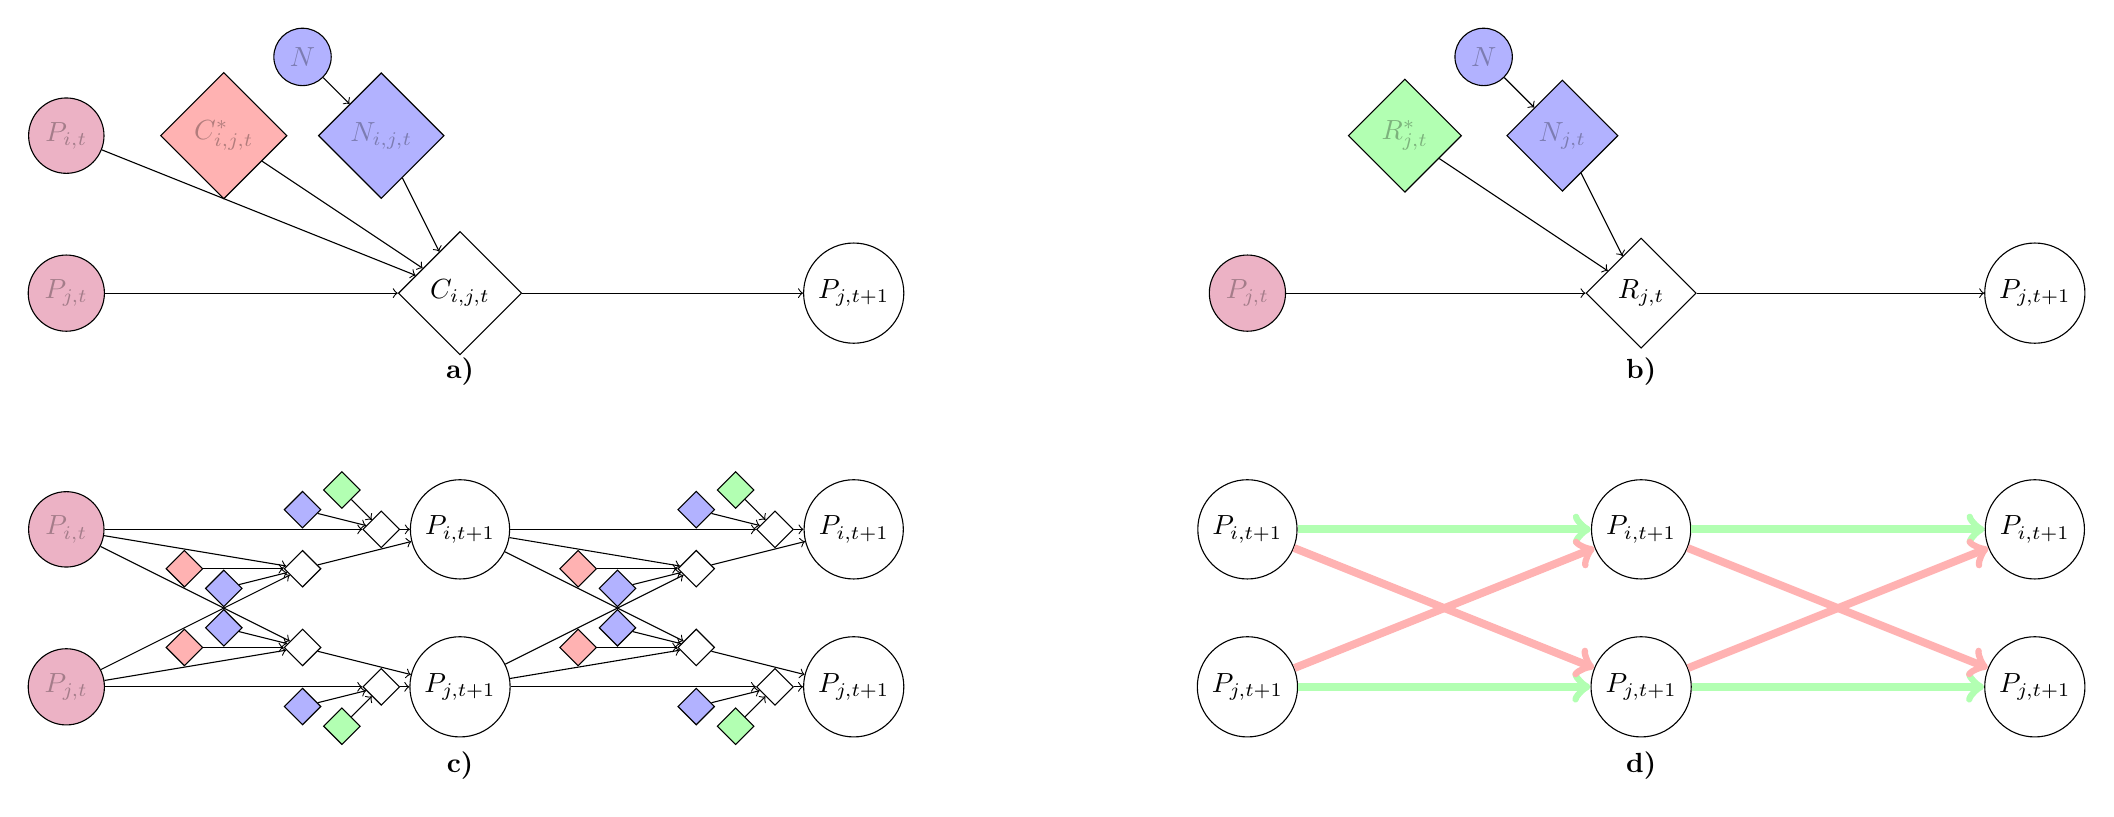
\begin{tikzpicture}
  %% Infectious Contacts
  \draw (-15,2) node[initial, node] (P11) {$P_{i,t}$};
  \draw (-15,0) node[initial, node] (P21) {$P_{j,t}$};
  \draw (-13,2) node[contact, edge] (E121) {$C^*_{i,j,t}$};
  \draw (-12,3) node[intervention, node] (I) {$N$};
  \draw (-11,2) node[intervention, edge] (I121) {$N_{i,j,t}$};
  \draw (-5,0) node[node] (P22) {$P_{j,t+1}$};
  \draw (-10,0) node[ edge] (C121) {$C_{i,j,t}$};
  
  \draw[->] (P11) -- (C121);
  \draw[->] (P21) -- (C121);
  \draw[->] (C121) -- (P22);
  \draw[->] (E121) -- (C121);
  \draw[->] (I121) -- (C121);
  \draw[->] (I) -- (I121);
  
  
  %% Recovery
  \draw (0,0) node[initial, node] (P21) {$P_{j,t}$};
  \draw (2,2) node[recovery, edge] (E121) {$R^*_{j,t}$};
  \draw (3,3) node[intervention, node] (I) {$N$};
  \draw (4,2) node[intervention, edge] (I11) {$N_{j,t}$};
  \draw (10,0) node[node] (P22) {$P_{j,t+1}$};
  \draw (5,0) node[ edge] (R121) {$R_{j,t}$};
  
  \draw[->] (P21) -- (R121);
  \draw[->] (R121) -- (P22);
  \draw[->] (E121) -- (R121);
  \draw[->] (I11) -- (R121);
  \draw[->] (I) -- (I11);
  
  
  %% Full
  \draw (-15,-3) node[initial, node] (P11) {$P_{i,t}$};
  \draw (-15,-5) node[initial, node] (P21) {$P_{j,t}$};

  \draw (-10,-3) node[node] (P12) {$P_{i,t+1}$};
  \draw (-10,-5) node[node] (P22) {$P_{j,t+1}$};

  \draw (-5,-3) node[node] (P13) {$P_{i,t+1}$};
  \draw (-5,-5) node[node] (P23) {$P_{j,t+1}$};

  %%% Contact edges
  \draw (-13.5,-4.5) node[contact, edge] (E121) {};
  \draw (-13.5,-3.5) node[contact, edge] (E211) {};
  \draw (-12,-4.5) node[ edge] (C121) {};
  \draw (-12,-3.5) node[ edge] (C211) {};
  \draw (-13,-4.25) node[intervention, edge] (I121) {};
  \draw (-13,-3.75) node[intervention, edge] (I211) {};
  
  \draw (-11.5,-5.5) node[recovery, edge] (E21) {};
  \draw (-12,-5.25) node[intervention, edge] (I21) {};
  \draw (-11,-5) node[edge] (R21) {};
  \draw (-11.5,-2.5) node[recovery, edge] (E11) {};
  \draw (-12,-2.75) node[intervention, edge] (I11) {};
  \draw (-11,-3) node[edge] (R11) {};


  \draw (-8.5,-4.5) node[contact, edge] (E122) {};
  \draw (-8.5,-3.5) node[contact, edge] (E212) {};
  \draw (-7,-4.5) node[ edge] (C122) {};
  \draw (-7,-3.5) node[ edge] (C212) {};
  \draw (-8,-4.25) node[intervention, edge] (I122) {};
  \draw (-8,-3.75) node[intervention, edge] (I212) {};
  
  \draw (-6.5,-5.5) node[recovery, edge] (E22) {};
  \draw (-7,-5.25) node[intervention, edge] (I22) {};
  \draw (-6,-5) node[edge] (R22) {};
  \draw (-6.5,-2.5) node[recovery, edge] (E12) {};
  \draw (-7,-2.75) node[intervention, edge] (I12) {};
  \draw (-6,-3) node[edge] (R12) {};


  \draw[->] (P11) -- (C121);
  \draw[->] (P21) -- (C121);
  \draw[->] (E121) -- (C121);
  \draw[->] (I121) -- (C121);
  \draw[->] (C121) -- (P22);

  \draw[->] (P11) -- (C211);
  \draw[->] (P21) -- (C211);
  \draw[->] (E211) -- (C211);
  \draw[->] (I211) -- (C211);
  \draw[->] (C211) -- (P12);

  \draw[->] (P11) -- (R11);
  \draw[->] (P21) -- (R21);
  \draw[->] (E11) -- (R11);
  \draw[->] (E21) -- (R21);
  \draw[->] (I11) -- (R11);
  \draw[->] (I21) -- (R21);
  \draw[->] (R11) -- (P12);
  \draw[->] (R21) -- (P22);
  
  
  
  \draw[->] (P12) -- (C122);
  \draw[->] (P22) -- (C122);
  \draw[->] (E122) -- (C122);
  \draw[->] (I122) -- (C122);
  \draw[->] (C122) -- (P23);

  \draw[->] (P12) -- (C212);
  \draw[->] (P22) -- (C212);
  \draw[->] (E212) -- (C212);
  \draw[->] (I212) -- (C212);
  \draw[->] (C212) -- (P13);

  \draw[->] (P12) -- (R12);
  \draw[->] (P22) -- (R22);
  \draw[->] (E12) -- (R12);
  \draw[->] (E22) -- (R22);
  \draw[->] (I12) -- (R12);
  \draw[->] (I22) -- (R22);
  \draw[->] (R12) -- (P13);
  \draw[->] (R22) -- (P23);

  \draw (0,-3) node[node] (P11) {$P_{i,t+1}$};
  \draw (0,-5) node[node] (P21) {$P_{j,t+1}$};

  \draw (5,-3) node[node] (P12) {$P_{i,t+1}$};
  \draw (5,-5) node[node] (P22) {$P_{j,t+1}$};

  \draw (10,-3) node[node] (P13) {$P_{i,t+1}$};
  \draw (10,-5) node[node] (P23) {$P_{j,t+1}$};

  \draw[->,line width=1mm, green!30!white] (P11) -- (P12);
  \draw[->,line width=1mm, green!30!white] (P21) -- (P22);
  \draw[->,line width=1mm, red!30!white] (P11) -- (P22);
  \draw[->,line width=1mm, red!30!white] (P21) -- (P12);

  \draw[->,line width=1mm, green!30!white] (P12) -- (P13);
  \draw[->,line width=1mm, green!30!white] (P22) -- (P23);
  \draw[->,line width=1mm, red!30!white] (P12) -- (P23);
  \draw[->,line width=1mm, red!30!white] (P22) -- (P13);

  %% Caption thingies
  \draw (-10,-1) node{\textbf{a)}};
  \draw (5,-1) node{\textbf{b)}};
  \draw (-10,-6) node{\textbf{c)}};
  \draw (5,-6) node{\textbf{d)}};
\end{tikzpicture}


\end{document}
